% Tipo de documento, tipo de papel, tamaño de letra
\documentclass[a4paper,11pt]{article}

% -----------------------------------------------------

% PAQUETES

% Paquete para usar reglas de castellano
\usepackage[spanish]{babel}
% Paquete para usar codificación UTF-8
\usepackage[utf8]{inputenc}
% Paquete para cambiar los márgentes
\usepackage{anysize}
%Fijar márgenes
\marginsize{2cm}{2cm}{2cm}{2cm}
% Paquete para insertar hipervínculos
\usepackage{hyperref}
% Paquete para poner color a las tablas
\usepackage[table,xcdraw]{xcolor}
% Paquete para insertar imágenes
\usepackage{graphicx}
\usepackage{float}
% Paquete para usar varias columnas
\usepackage{multicol}
% Paquete para usar enumerados
\usepackage{enumerate}
% Paquete para fuentes matemáticas
\usepackage{dsfont}
\usepackage{amsfonts}
\usepackage{amsmath}
\usepackage{textcomp}

% Ruta de las imágenes
\graphicspath{C:\Users\angfd\Desktop\Git}
\marginsize{2cm}{2cm}{2cm}{2cm}

% -----------------------------------------------------
\begin{document}
	
\begin{titlepage}
	\title{\textbf{Proyecto Final. Curso Latex. Valoración nutricional: Parámetros antropométricos y bioquímicos}}
	\author{Ángel Fernández-Aparicio}
	\date{\today}
	\maketitle
\end{titlepage}
	
\tableofcontents
\newpage

\begin{abstract}
Todos los documentos relativos al proyecto se encuentran disponibles en el siguiente repositorio de \textbf{Github:} \href{https://github.com/anfeapa/proyecto_final}{URL del repositorio}.
		
El objetivo del presente documento es realizar un proyecto final del curso LaTeX y Git aplicado a las investigaciones científicas. Para ello, se desarrollarán los conocimientos adquiridos con el fin de:\begin{enumerate}
	\item Crear un repositorio público.
	\item Crear un documento \textbf{LaTeX }similar al utilizado en las publicaciones científicas.
	\item Usar el repositorio creado en \textbf{GitHub} para controlar y documentar la redacción del artículo.
	\end{enumerate} 
\end{abstract}
	
\section{Introducción}
La valoración nutricional permite detectar y prevenir el riesgo de malnutrición, ya sea por exceso (sobrepeso u obesidad) o por defecto (desnutrición). Esta valoración también permite adecuar la dieta a las necesidades de los seres humanos, por ende se puede reducir así la aparición de malnutrición o sobrepeso/obesidad y sus consecuentes complicaciones. 

Existen diferentes herramientas para realizar la valoración nutricional como sería la historia dietética, determinación de parámetros antropométricos, análisis de la composición corporal mediante bioimpedancia eléctrica, análisis de parámetros bioquímicos, cuestionarios, etc. 

En este proyecto se van a listar algunos de los parámetros antropométricos, así como algunos de los parámetros bioquímicos que se pueden analizar y son importantes en la valoración nutricional. 

\section{Antropometría vs Parámetros Bioquímicos/Impedancia}
A continuación en la presente sección se compararán dos listas, enfrentadas entre sí, mencionando parámetros antropométricos y parámetros bioquímicos/inmunológicos/impedancia: 
	
\begin{minipage}[l]{0.5\linewidth}
	\begin{itemize}
	\item Peso
	\item Talla
	\item IMC
	\item Índice Cintura-Cadera
	\item Pliegues cutáneos
	\end{itemize}
\end{minipage}
\begin{minipage}[r]{0.5\linewidth}
	\begin{itemize}
	\item Niveles de albúmina
	\item Niveles de prealbúmina
	\item Recuento total linfocitario
	\item Grasa corporal
	\item Agua corporal
	\end{itemize}
\end{minipage}

\section{Imágenes y tablas}
\subsection{Imágenes}
Introducimos imagen: 
\begin{figure}[H]
	\centering
	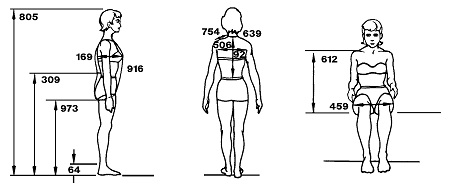
\includegraphics[width=0.5\linewidth]{antro}
	\caption{Antropometría}
	\label{Fig 2: Antropometría}
\end{figure}

\subsection{Tablas}
	Introducimos la siguiente tabla:
		
\begin{center}
	\ Clasificación de la Obesidad según el IMC. Criterios SEEDO, 2007\
\end{center}
		
\begin{table}[H]
	\begin{center}
	\begin{tabular}{|c|c|c}
		\hline
		\rowcolor[HTML]{C0C0C0} 
		{\color[HTML]{333333} \textbf{CATEGORÍA}} & {\color[HTML]{333333} \textbf{IMC (kg/m2})} \\ \hline
		Peso Insuficiente                & \textless 18,5                    \\ \hline
		Normopeso                        & 18,5-24,9                         \\ \hline
		\multicolumn{2}{|c|}{\textbf{SOBREPESO}}                                      \\ \hline
		Grado I                          & 25,0-26,9                         \\ \hline
		Grado II                         & 27,0-29,9                         \\ \hline
		\multicolumn{2}{|c|}{\textbf{OBESIDAD}}                                       \\ \hline
		Tipo I                           & 30,0-34,9                         \\ \hline
		Tipo II                          & 35,0-39,9                         \\ \hline
		Tipo III (mórbida)               & 40,0-49,9                         \\ \hline
		Tipo IV (extrema)                & $\geq$ 50                       \\ \hline
	\end{tabular}
	\end{center}
	\end{table}
		
\section{Fórmulas}
A continuación se describen las fórmulas matemáticas que permiten el cálculo de los parámetros antropométricos Abdominal Volume Index (AVI), Índice Cintura-Cadera (ICC), Body Adiposity Index (BAI) and Body Shape Index (ABSI). Dichas fórmulas las crearemos tanto en línea como usando <<equation>>.
		
\subsection{Fórmulas en línea}
\begin{itemize}
	\item ICC: $$ICC= WC/HC$$
	\item BAI: $$BAI = [HC(m)/Height^{\frac{2}{3}}(m)]-18$$
			
\end{itemize}
	
Abreviaturas: Circunferencia de la Cintura (WC), Circunferencia de la Cadera (HC) e Índice de Masa Corporal (BMI)
		
\subsection{Fórmulas usando <<equation>>}
 \begin{equation}
	AVI = (2WC^{2}(cm)+ 0.7 (WC-HP)^{2}(cm))\div 1000
 \end{equation}
		
 \begin{equation}
	BAI = [HC(m)/Height^{\frac{2}{3}}(m)]-18
 \end{equation}
		
 \begin{equation}
    ABSI = WC(m)/(BMI^{\frac{2}{3}}(kg/m^{2})Height^{\frac{1}{2}}(m))
 \end{equation}
		
Abreviaturas: Circunferencia de la Cintura (WC), Circunferencia de la Cadera (HC) e Índice de Masa Corporal (BMI)
		
	\bibliography{M6_Fernandez_Aparicio_Angel}
	\bibliographystyle{plain}
	\nocite{*}
		
\end{document}